%!TEX root = ../thesis.tex
%*******************************************************************************
%****************************** Second Chapter *********************************
%*******************************************************************************

\chapter{Estado del Arte}

\ifpdf
    \graphicspath{{Chapter2/Figs/Raster/}{Chapter2/Figs/PDF/}{Chapter2/Figs/}}
\else
    \graphicspath{{Chapter2/Figs/Vector/}{Chapter2/Figs/}}
\fi

\section{Términos relacionados con el estilo de conducción}

El concepto de "Estilo de conducción" no tiene una definición estándar que sea aceptada en todo el mundo. Al contrario, este concepto involucra una serie de factores que aumentan su complejidad y complican su definición. Debido a esto se usarán los conceptos definidos por \citeauthor{8002632} \cite{8002632}.

\begin{figure}[htbp!]
\centering
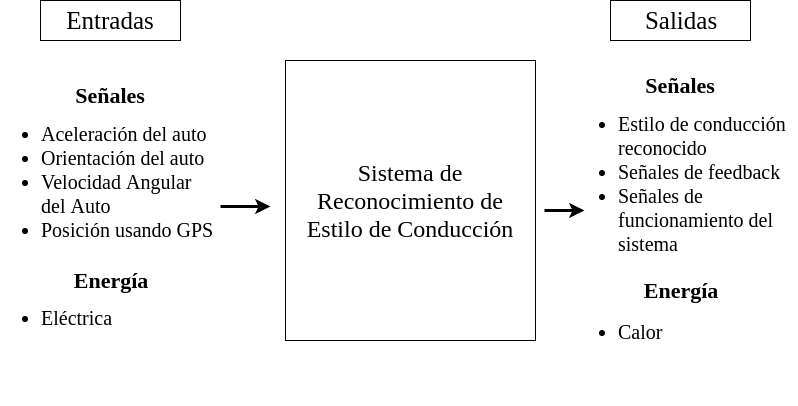
\includegraphics[width=0.8\textwidth]{Fig1}
\caption[Terminología estilo de conducción]{Terminología relacionada con el estilo de conducción \cite{8002632}}
\label{fig:2.1}
\end{figure}

Como se aprecia en la Fig~\ref{fig:2.1}, se entiende por un evento de conducción como las maniobras que se usan durante la acción de conducir, como por ejemplo: acelerar, desacelerar y girar.

De la misma manera, El patrón de conducción se define como el resultado de los eventos de conducción sujetos a condiciones de manejo, como el clima o el tipo de calzada. Este resultado se puede expresar como un perfil de velocidades. en el que están incluidos todos los datos que se pueden obtener partiendo de este perfil de velocidad, como por ejemplo: duración del viaje, velocidad promedio y demanda de potencia calculada.

La habilidad de conducción, es la habilidad que posee el conductor para controlar el vehículo. Este concepto se usa para diferenciar entre un conductor experimentado o profesional de un conductor promedio.

El estilo de conducción es más complejo de definir debido a que para algunos autores involucra factores subjetivos como la actitud del conductor, el humor o el cansancio. Para \citeauthor{6957822} \cite{6957822}, el estilo de conducción  es la manera en la que la tarea de conducción es realizada. Esto se traduce a la forma en la que el conductor opera el vehículo (Pedal de aceleración, timón, freno, etc.). Esto se diferencia de el patrón de conducción tan solo porque no se asocia con un recorrido en especifico sino con el conductor.

También se puede expresar el estilo de conducción en niveles de agresividad como \citeauthor{6294318} \cite{6294318}. Como la agresividad en los eventos de conducción esta asociada con un mayor consumo de combustible y a menor seguridad vial, definitivamente juega aun papel importante dentro del concepto de estilo de conducción. \mynote{Se debe definir cual es el concepto que se manejará en la tesis}

\section{Estado del arte según algoritmos usados}
Se procederá a mostrar las implementaciones e investigaciones desarrolladas en la actualidad clasificados según el tipo de algoritmo que se uso para la caracterización de el estilo de conducción

\subsection{Algoritmos basados en reglas}
Dentro de esta categoría se encuentran algoritmos de clasificación basados en reglas que comprenden el uso de lógica difusa, lógica difusa adaptativa y algoritmos de agrupamiento. Estos algoritmos se caracterizan por estar definidos por {\it umbrales predefinidos} y son el enfoque más sencillo para tratar de clasificar los estilos de conducción.

\citeauthor{6957822} \cite{6957822} desarrolló un sistema de reconocimiento de estilo de conducción online usando lógica difusa. Este sistema esta implementado usando {\it Matlab/Simulink}  y es paramétrico, Se puede configurar para ser usado en distintos tipos de vehículos.
El sistema detecta la aceleración longitudinal, aceleración lateral, desaceleración, velocidad, brecha de tiempo y activación del sistema autónomo de velocidad crusero. Además determina a través de un Sistema de Navegación el tipo de calzada en el que se encuentra (Se distingue entre trocha, calles urbanas, carreteras pavimentadas y carreteras rurales). Esto lo realiza debido a que el tipo de calzada influencia en gran medida al estilo de conducción. Por ejemplo, en una trocha la mayoría de conductores manejarían a una velocidad suave para no dañar al vehículo, lo cuál no necesariamente quiere decir que el mismo conductor conduzca de esa manera en otro tipo de escenarios.
Usando Lógica Difusa se definieron 3 niveles de estilo de conducción: {\it Normal, Confortable y Deportivo}. Se probó el sistema en una simulación y se obtuvieron los siguientes resultados promedio (Fig.~\ref{fig:2.2}): 67.8\% de clasificaciones correctas y solo 2\% de clasificaciones incorrectas (El otro 30.2\% pertenece a clasificaciones "Diferentes" que dan una clasificación contigua de estilo de manejo, por ejemplo cuando la clasificación real es {\it Normal} pero el sistema arroja como resultado {\it Confortable}, en cambio las clasificaciones incorrectas dan un resultado no contiguo al real)

\begin{figure}[htbp!]
\centering
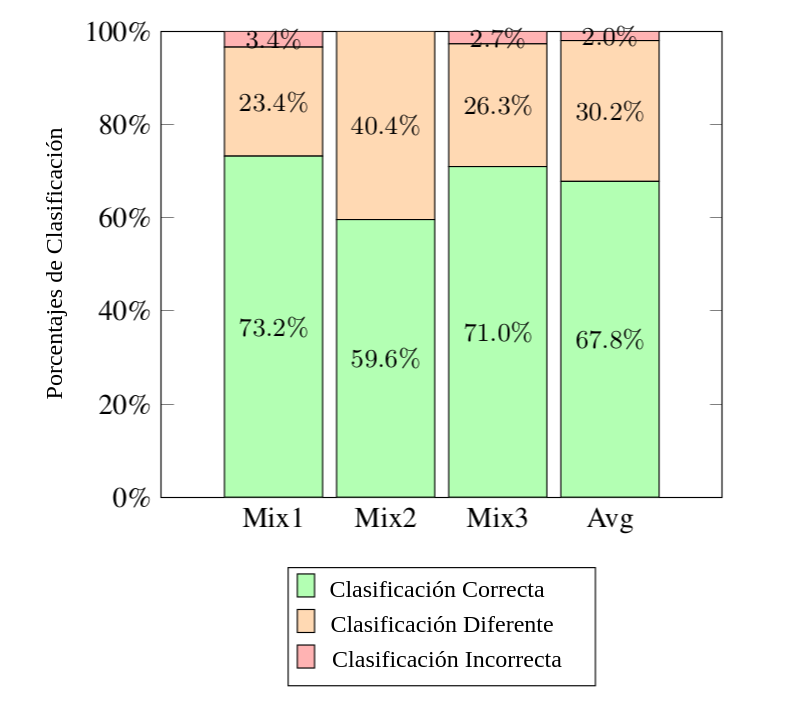
\includegraphics[width=0.8\textwidth]{Fig2}
\caption[Terminología estilo de conducción]{Resultados del sistema de reconocimiento de estilo de conducción en \cite{6957822}}
\label{fig:2.2}
\end{figure}

Usar lógica difusa no es la única manera de clasificar estilos de conducción. \citeauthor{4938719} \cite{4938719} presentó un método de clasificación basado en el análisis del perfil de la sobreaceleración (la derivada de la aceleración respecto al tiempo). En su investigación define al estilo de manejo como un comportamiento dinámico, Un conductor puede manejar de forma calmada por un momento y de forma agresiva en otro momento. Por este motivo el método de clasificación que propone predice el estilo de conducción del usuario en tiempo real. 
El algoritmo funciona de la siguiente manera:
\begin{enumerate}
    \item Calcula el perfil de sobreaceleración durante una ventana de tiempo predefinido.
    \item Calcula la desviación estándar de la sobreaceleración durante toda la ventana de tiempo.
    \item Detecta el tipo de calzada actual y el nivel de congestión de tráfico usando el algoritmo propuesto en \cite{Highway_cap_manual}.
    \item Calcula la proporción de sobreaceleración dividiendo la desviación estándar con un valor promedio que depende de el tipo de calzada y el nivel de tráfico actuales.
    \item Dependiendo del resultado de la división realizada el conductor puede ser clasificado como {\it Calmado, Normal} o {\it Agresivo} usando reglas con umbrales predefinidos.
\end{enumerate}
\begin{figure}[H]
\centering
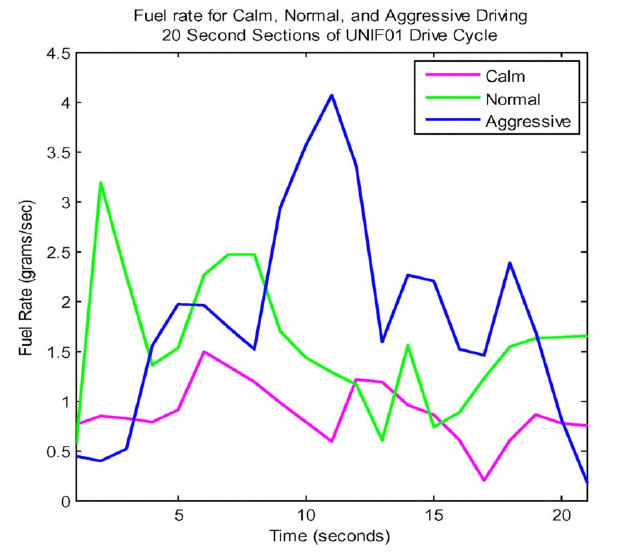
\includegraphics[width=0.7\textwidth]{Fig3}
\caption{Tasa de consumo de combustible según diferentes estilos de conducción \cite{4938719}.}
\label{fig:2.3}
\end{figure}
Este resultado dependerá mucho de la duración definida para la ventana de tiempo. Se recomendó usar una ventana de duración de 6 a 9 segundos para detectar los cambios de estilo de conducción oportunamente.

Se realizó también una comparación entre los 3 diferentes estilos de conducción con respecto a la tasa de consumo de combustible. Como se puede apreciar en la Fig.~\ref{fig:2.3}, los conductores clasificados como calmados están asociados a un menor consumo de combustible, mientras que los agresivos a un mayor consumo de combustible.

%para optimizar el uso de combustible. Por ejemplo en un vehículo híbrido, si el sistema predice que el conductor manejará de una manera agresiva, el sistema usará más potencia del motor eléctrico que del de combustión para así ayudar al ahorro de combustible.

Se ha presentado dos algoritmos basados en reglas que usan tanto múltiples variables \cite{6957822} como una sola \cite{4938719} para predecir el estilo de conducción del usuario. Sin embargo, los resultados de estos sistemas dependen en gran medida del valor de los umbrales escogidos para realizar la clasificación.

\section{Algoritmos basados en Datos}
Cuando se tiene una cantidad muy grande de datos, es difícil analizarlos para obtener las reglas que guíen al algoritmo. Es entonces cuando los algoritmos basados en datos entran en acción. Estos algoritmos, en comparación con los basados en reglas, pueden manejar una mayor cantidad de datos y deducir umbrales consistentes con estos datos sin que estos dependan de un experto en el tema. A continuación se presentarán los distintos tipos de algoritmos basados en datos y su uso en el reconocimiento de estilos de conducción.

\subsection{Algoritmos de aprendizaje de máquinas no supervisados}
Los algoritmos no supervisados no necesitan que los datos obtenidos por medio de los sensores en la actividad de conducción estén etiquetados. Es decir

